\begin{figure}[bth!]
	\begin{center}
	   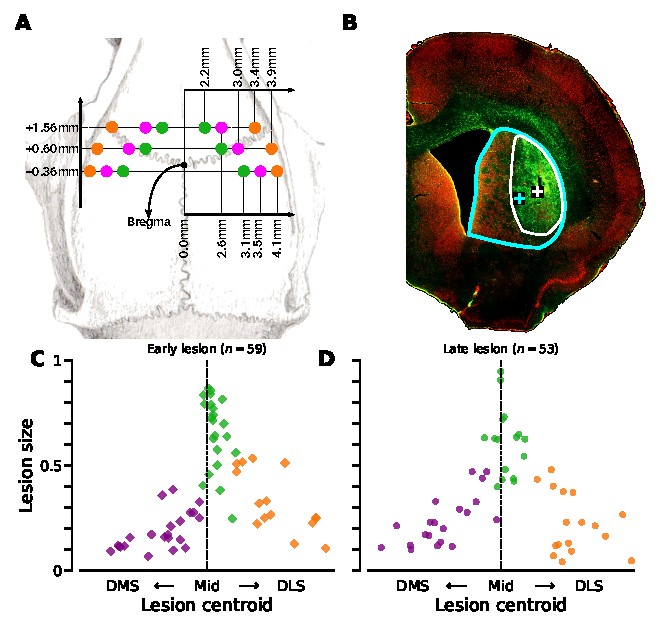
\includegraphics[scale=1]{ch-methods/figures/LesionSizeLocation.pdf}
	   \caption
	   {\textbf{Dorsal striatum lesion quantification.}
	   \textbf{(A)} Schematic of the lesion sites.
	   \textbf{(B)} Illustration of the quantification of the lesion size. For each coronal slide and hemi-striatum, the contour of the lesion was manually outlined using GFAP staining.
	   The relative size of the lesion (compared to the full dS, manually outlined on the NeuN staining) and the coordinates of the lesion/striatum centroid was calculated.
	   For each animal, the size and laterality were obtained by averaging data along the anteroposterior axis, for both left and right hemispheres.
	   \textbf{(C, D)} Lesion size versus laterality for animals that underwent lesion before (Early, C) and after (Late, D) extensive practice.
	   Lesion quantification was performed blindly relative to behavioral analysis.
   In four animals with a dS lesion performed after learning the task (late lesion), the lesion size quantification could not be properly performed.
	   These animals were classified according to their injection coordinates in the surgery (3 DLS and 1 DMS), however they were excluded from any analyses that required the lesion size (hence the difference between the number of "late lesion" animals in this figure, $n=53$, and the total number of animals in Fig.~1, $n=57$).
	   }
	   \label{fig:method:LesionSizeLocation}
	\end{center}
   \end{figure}